\documentclass[14pt]{beamer}

\usepackage[english]{babel}
\usepackage[utf8x]{inputenc}

\usetheme{m}
\usepackage{pacman}
\usefonttheme{structurebold}
\setbeamercovered{transparent}


\usepackage{listings}
\definecolor{darkgreen}{rgb}{0,0.6,0}
\lstset{
    basicstyle=\ttfamily,
    showstringspaces=false,
    commentstyle=\color{red},
    keywordstyle=\color{blue},
    stringstyle=\color{darkgreen}
}
\makeatletter
\lstdefinelanguage{llvm}{
  morecomment = [l]{;},
  morestring=[b]", 
  sensitive = true,
  classoffset=0,
  morekeywords={
  },
  classoffset=1, keywordstyle=\color[rgb]{0.228, 0.703, 0.718},
  morekeywords={
    % instructions
    % terminators
    ret, br, switch, indirectbr, invoke, resume, unreachable,
    % binary operations
    add, fadd, sub, fsub, mul, fmul, udiv, sdiv, fdiv, urem, srem, frem,
    % bitwise binary operations
    shl, lshr, ashr, and, or, xor,
    % vector operations
    extractelement, insertelement, shufflevector,
    % aggregate operations
    extractvalue, insertvalue,
    % memory access and addressing operations
    alloca, load, store, fence, cmpxchg, atomicrmw, getelementptr,
    % conversion operations
    trunc, zext, sext, fptrunc, fpext, fptoui, fptosi, uitofp, sitofp, ptrtoint,
    inttoptr, bitcast,
    % other operations
    icmp, fcmp, phi, select, call, va_arg, landingpad,
    % instruction arguments
    nuw, nsw, exact, acquire, release, acq_rel, seq_cst, singlethread, volatile,
    xchg, add, sub, and, nand, or, xor, max, min, umax, umin, to, eq, ne, ugt,
    uge, ult, ule, sgt, sge, slt, sle, false, oeq, ogt, oge, olt, ole, one, ort,
    ueq, ugt, uge, ult, ule, une, uno, true,  personality, catch, filter,
    cleanup, inbounds, unwind, label, align, tail, to,
    % I thought these shouldn't be the same color as %vars, moved from
    % lower-level keywords
    define, declare, global, constant,
    internal, external, private,
    linkonce, linkonce_odr, weak, weak_odr, appending,
    common, extern_weak,
    thread_local, dllimport, dllexport,
    hidden, protected, default,
    except, deplibs,
    volatile, fastcc, coldcc, cc, ccc,
    x86_stdcallcc, x86_fastcallcc,
    ptx_kernel, ptx_device,
    signext, zeroext, inreg, sret, nounwind, noreturn,
    nocapture, byval, nest, readnone, readonly, noalias, uwtable,
    inlinehint, noinline, alwaysinline, optsize, ssp, sspreq,
    noredzone, noimplicitfloat, naked, alignstack,
    module, asm, align, tail, to,
    addrspace, section, alias, sideeffect, c, gc,
    target, datalayout, triple,
    blockaddress
  },
  alsoletter={\%,.},
  keywordsprefix={\%},
}
\makeatother

%%
% from http://tex.stackexchange.com/questions/23647/drawing-a-directory-listing-a-la-the-tree-command-in-tikz
\usepackage{forest}
\usetikzlibrary{arrows.meta}
\forestset{
  dir tree/.style={
    for tree={
      parent anchor=south west,
      child anchor=west,
      anchor=mid west,
      inner ysep=1pt,
      grow'=0,
      align=left,
      edge path={
        \noexpand\path [draw, \forestoption{edge}] (!u.parent anchor) ++(1em,0) |- (.child anchor)\forestoption{edge label};
      },
      font=\sffamily,
      if n children=0{}{
        delay={
          prepend={[,phantom, calign with current]}
        }
      },
      fit=band,
      before computing xy={
        l=2em
      }
    },
  }
}

%%

\newcommand{\Command}[1]{\textbf{\texttt{#1}}}
\newcommand{\Code}[1]{\textbf{\texttt{#1}}}

%%

\title{Building, Testing and Debugging a Simple out-of-tree LLVM Pass}
\date{October 29, 2015, LLVM Developers' Meeting}

\begin{document}

{
    \logo{
\includegraphics[height=5em]{logo.png}\hspace{2em}}
	\begin{frame}
        \maketitle
	\end{frame}
}

    %%%%%%%%%%%%%%%%%%%%%%%%%%%%%%%%%%%%%%%
    %%%%%%%%%%%%%%%%%%%%%%%%%%%%%%%%%%%%%%%
    %%%%%%%%%%%%%%%%%%%%%%%%%%%%%%%%%%%%%%%

    \begin{frame}{LLVM 3.7 --- Resources}
        \begin{center}
            \url{https://github.com/quarkslab/llvm-dev-meeting-tutorial-2015}
        \end{center}
    \end{frame}

    %%%%%%%%%%%%%%%%%%%%%%%%%%%%%%%%%%%%%%%
    %%%%%%%%%%%%%%%%%%%%%%%%%%%%%%%%%%%%%%%
    %%%%%%%%%%%%%%%%%%%%%%%%%%%%%%%%%%%%%%%

    \begin{frame}{LLVM 3.7 --- Tutorial}
        \begin{center}
            \textbf{\Large Press Start Button}
        \end{center}
    \end{frame}

    \begin{frame}{LLVM 3.7 --- Prerequisite}
        \begin{center}
            \textbf{\Large Please Load LLVM3.7}
        \end{center}
    \end{frame}

    \begin{frame}{LLVM 3.7}
        \begin{center}
            \begin{itemize}
                \centering
                \item[]\alert{\bf Select difficulty}\vspace{1em}
                \item[] \textbf{\texttt{>~}Easy\texttt{~<}}
                \item[] Hard
                \item[] Nightmare
            \end{itemize}
        \end{center}
    \end{frame}

    \begin{frame}{LLVM 3.7}

            \begin{itemize}
                \centering
                \item[]\alert{\bf Stage Selection}\vspace{1em}
                \item[] Adding a new Front-End
                \item[] In-Tree Pass Development
                \item[] \textbf{\texttt{>~}Out-of-Tree Pass Development\texttt{~<}}
                \item[] Adding a new Back-End
            \end{itemize}

    \end{frame}

    \begin{frame}{LLVM 3.7}

            \begin{itemize}
                \centering
                \item[]\alert{\bf OS Selection}\vspace{1em}
                \item[] \textbf{\texttt{>~}Linux\texttt{~<}}
                \item[] OSX
                \item[] \tikz\node[opacity=0.5]{Windows};
            \end{itemize}

    \end{frame}

    %%%%%%%%%%%%%%%%%%%%%%%%%%%%%%%%%%%%%%%
    %%%%%%%%%%%%%%%%%%%%%%%%%%%%%%%%%%%%%%%
    %%%%%%%%%%%%%%%%%%%%%%%%%%%%%%%%%%%%%%%

    \begin{frame}{stage 1}

        \framesubtitle{Setup a Proper CMake Project}

        \begin{block}{Goals}
            \begin{itemize}
                \item Use LLVM Cmake support
                \item Build a minimal pass
            \end{itemize}

        \end{block}

        \begin{alertblock}{Bonus}
            \begin{itemize}
                \item Setup a minimal test driver
                \item Make the pass compatible with \Command{clang}
            \end{itemize}
        \end{alertblock}

    \end{frame}

    \begin{frame}{stage 1 --- Directory Layout}
    \begin{forest}
          dir tree
          [Tutorial
              [CMakeLists.txt\only<2>{\usebeamercolor[fg]{alerted text}~$\longleftarrow$ CMake configuration file}]
              [cmake\only<3>{\usebeamercolor[fg]{alerted text}~$\longleftarrow$ CMake auxiliary files}
                [Python.cmake]
              ]
              [MBA\only<4>{\usebeamercolor[fg]{alerted text}~$\longleftarrow$ Our first pass}
                  [CMakeLists.txt]
                  [MBA.cpp]
              ]
          ]
    \end{forest}
    \end{frame}

    \begin{frame}[containsverbatim]
        \frametitle{stage 1 --- \texttt{CMakeLists.txt}}
        \begin{block}{LLVM Detection}
            \footnotesize
            \lstinputlisting[firstline=5, lastline=11,language=bash,morekeywords={endif,message}]{../CMakeLists.txt}
        \end{block}
    \end{frame}

    \begin{frame}[containsverbatim]
        \frametitle{stage 1 --- \texttt{CMakeLists.txt}}
        \begin{block}{Load LLVM Config}
            \footnotesize
            \lstinputlisting[firstline=15, lastline=17,language=bash,morekeywords={list,find_package}]{../CMakeLists.txt}
        \end{block}
        \begin{block}{And more LLVM Stuff}
            \footnotesize
            \lstinputlisting[firstline=19, lastline=21,language=bash,morekeywords={list,include}]{../CMakeLists.txt}
        \end{block}
    \end{frame}

    \begin{frame}[containsverbatim]
        \frametitle{stage 1 --- \texttt{CMakeLists.txt}}
        \begin{block}{Propagate LLVM setup to our project}
            \footnotesize
            \lstinputlisting[firstline=24, lastline=27,language=bash,morekeywords={add_definitions,include_directories}]{../CMakeLists.txt}
        \end{block}

        \begin{block}{Get Ready!}
            \footnotesize
            \lstinputlisting[firstline=34, lastline=34,language=bash,morekeywords={add_subdirectory}]{../CMakeLists.txt}
        \end{block}
    \end{frame}

    \begin{frame}[containsverbatim]
        \frametitle{stage 1 --- \texttt{MBA/CMakeLists.txt}}
        \begin{block}{Declare a Pass}
            \footnotesize
            \lstinputlisting[firstline=2, lastline=2,language=bash,morekeywords={add_llvm_loadable_module}]{../MBA/CMakeLists.txt}
        \end{block}

        \begin{alertblock}{1 Pass = 1 Dynamically Loaded Library}
            \begin{itemize}
                \item Passes are loaded by a pass driver: \textbf{\texttt{opt}}
{
\footnotesize
\begin{lstlisting}[language=bash]
% opt -load LLVMMBA.so -mba input.ll -S
\end{lstlisting}
}
                \item Or by clang (provided an extra setup)
{
\footnotesize
\begin{lstlisting}[language=bash]
% clang -Xclang -load -Xclang LLVMMBA.so input.c -c
\end{lstlisting}
}
            \end{itemize}
        \end{alertblock}

    \end{frame}

    \begin{frame}[containsverbatim]
        \frametitle{stage 1 --- \texttt{MBA.cpp}}
        {
            \footnotesize
            \lstinputlisting[linerange={24-24,27-27,45-45,52-55,58-58,60-60,71-72,111-113},language=c++]{../MBA/MBA.cpp}
        }
    \end{frame}


    \begin{frame}[containsverbatim]
        \frametitle{stage 1 --- \texttt{MBA.cpp}}
        \begin{alertblock}{Registration Stuff}
            \begin{itemize}
                \item Only performs registration for \Command{opt} use!
                \item Uses a static constructor\dots
            \end{itemize}
        \end{alertblock}
        {
            \footnotesize
            \lstinputlisting[linerange={130-138},language=c++]{../MBA/MBA.cpp}
        }
    \end{frame}

    \begin{frame}[containsverbatim]
        \frametitle{stage 1 --- Bonus Level}
        \begin{alertblock}{Setup test infrastructure}
            \begin{itemize}
                \item Rely on \Command{lit}, LLVM's Integrated Tester
                \item {\footnotesize
\begin{lstlisting}[language=bash]
% pip install --user lit
\end{lstlisting}
                    }
            \end{itemize}
        \end{alertblock}

        \begin{block}{\texttt{CMakeLists.txt} update}
{
\scriptsize
\lstinputlisting[linerange={39-41,50-53},language=bash,morekeywords={list,include,find_python_module,REQUIRED,add_custom_target,COMMAND}]{../CMakeLists.txt}
}
        \end{block}
    \end{frame}

    \begin{frame}[containsverbatim]
        \frametitle{stage 1 --- Bonus Level}
        \begin{alertblock}{Make the pass usable from \Command{clang}}
            \begin{itemize}
                \item Automatically loaded in \Command{clang}'s optimization flow: {\footnotesize\lstinline|clang -Xclang -load -Xclang|}
                \item Several extension point exist
            \end{itemize}
        \end{alertblock}

{
\scriptsize
\lstinputlisting[linerange={142-147,151-152},language=bash,morekeywords={list,include,find_python_module,REQUIRED,add_custom_target,COMMAND}]{../MBA/MBA.cpp}
}
    \end{frame}

    %%%%%%%%%%%%%%%%%%%%%%%%%%%%%%%%%%%%%%%
    %%%%%%%%%%%%%%%%%%%%%%%%%%%%%%%%%%%%%%%
    %%%%%%%%%%%%%%%%%%%%%%%%%%%%%%%%%%%%%%%

    \begin{frame}{stage 2}

        \framesubtitle{Build a Simple Pass}

        \begin{block}{Goals}
            \begin{itemize}
                \item Learn basic LLVM IR manipulations
                \item Write a simple test case
            \end{itemize}

        \end{block}

        \begin{alertblock}{Bonus}
            \begin{itemize}
                \item Collect statistics on your pass
                \item Collect debug informations on your pass
            \end{itemize}
        \end{alertblock}

    \end{frame}

    \begin{frame}{stage 2 --- MBA}
        \framesubtitle{Mixed Boolean Arithmetic}

        \begin{alertblock}{Simple Instruction Selection}
            Turns: $a + b$

            Into: $(a \oplus b) + 2 \times (a \wedge b)$
        \end{alertblock}

        \begin{block}{Context}
            \alert{$\Rightarrow$} Useful for code obfuscation
        \end{block}

    \end{frame}

    \begin{frame}[containsverbatim]
    \frametitle{stage2 --- \texttt{runOnBasicBlock++}}
    \begin{itemize}
        \item Iterate over a \Code{BasicBlock}
        \item Use LLVM's \Code{dyn\_cast}
    \end{itemize}
    {
        \scriptsize
        \lstinputlisting[breaklines=true,linerange={75-75,79-79,83-84},language=c++]{../MBA/MBA.cpp}
    }
    \end{frame}

    \begin{frame}[containsverbatim]
    \frametitle{stage2 --- \texttt{runOnBasicBlock++}}
    LLVM Instruction creation/insertion:
    \begin{itemize}
        \item Use \Code{IRBuilder} from \Code{llvm/IR/IRBuilder.h}
    \end{itemize}
    \hspace{-5em}%
    \begin{minipage}{\textwidth}
        \scriptsize
        \lstinputlisting[breaklines=false,linerange={89-96},language=c++]{../MBA/MBA.cpp}
    \end{minipage}
    \end{frame}

    \begin{frame}[containsverbatim]
    \frametitle{stage2 --- \texttt{runOnBasicBlock++}}
    Instruction substitution:
    \begin{itemize}
		\item Use \Code{Value::replaceAllUsesWith}, but the old instruction has
			to be removed afterwards (safest)
		\item Use \Code{llvm::ReplaceInstWithValue} that does the job for you
			(need to be careful on iterator validity)
    \end{itemize}
    \hspace{-6em}%
    \begin{minipage}{\textwidth}
        \footnotesize
        \lstinputlisting[breaklines=false,linerange={114-114},language=c++]{../MBA/MBA.cpp}
    \end{minipage}
    \end{frame}

    \begin{frame}{stage 2 --- Write a simple test}
        \begin{alertblock}{\Command{lit} principles}
            \begin{itemize}
                \item One source file (say \texttt{.c} or \texttt{.ll}) per test case
                \item Use comments to describe the test
                \item Use substitution for test configuration
            \end{itemize}
        \end{alertblock}

        \begin{block}{\Command{FileCheck} --- \Command{grep} on steroids!}
            \begin{itemize}
                \item Compares \Code{argv[1]} and \Code{stdin}
                \item Reads check\textbf{s} from comments in \Code{argv[1]}
                \item[$\Rightarrow$] Requires LLVM with \Code{-DLLVM\_INSTALL\_UTILS}
            \end{itemize}
        \end{block}
    \end{frame}

    \begin{frame}[containsverbatim]{stage 2 --- test sample}
    \hspace{-1em}\begin{minipage}{\textwidth}
            \footnotesize
            \lstinputlisting[breaklines=true,language=c]{../Tests/MBA.c}
        \end{minipage}
    \end{frame}

    \begin{frame}[containsverbatim]{stage 2 --- advanced tests}
    \hspace{-1em}\begin{minipage}{\textwidth}
            \footnotesize
            \lstinputlisting[breaklines=true,linerange={1-7},language=llvm]{../Tests/MBA.ll}
            \dots
            \lstinputlisting[breaklines=true,linerange={22-22},language=llvm]{../Tests/MBA.ll}
        \end{minipage}
    \end{frame}


    \begin{frame}[containsverbatim]{stage 2 --- Bonus}
        \framesubtitle{Collect Statistics}
        \structure{How many substitutions have we done?}
        {
        \footnotesize
        \lstinputlisting[breaklines=true,linerange={21-22},language=c++]{../MBA/MBA.cpp}
        }
        \vspace{-1em}%
        \hspace{-5.5em}%
        \begin{minipage}{\textwidth}
            \footnotesize
            \lstinputlisting[breaklines=false,linerange={117-118},language=c++]{../MBA/MBA.cpp}
        \end{minipage}

        \structure{Collect them!}
        {
        \footnotesize
\begin{lstlisting}[language=bash]
% opt -load LLVMMBA.so -mba -stats ...
\end{lstlisting}
        }
    \end{frame}

    \begin{frame}[containsverbatim]{stage 2 --- Bonus}
        \framesubtitle{Debug your pass}
        \begin{alertblock}{\Code{DEBUG()} and \Code{DEBUG\_TYPE}}
        Setup a guard:
        {
        \footnotesize
        \lstinputlisting[breaklines=true,linerange={15-16},language=c++]{../MBA/MBA.cpp}
        }
        Add a trace:\\
        \hspace{-6em}%
        \begin{minipage}{\textwidth}
        \footnotesize
        \lstinputlisting[breaklines=false,linerange={101-101},language=c++]{../MBA/MBA.cpp}
        \end{minipage}
        \end{alertblock}
        \begin{block}{Collect the trace}
        {
        \footnotesize
        \begin{lstlisting}[language=bash]
% opt -O2 -mba -debug ... # verbose
% opt -O2 -mba -debug-only=mba ... # selective
        \end{lstlisting}
        }
        \end{block}
        Everything disapears under \Code{-DNDEBUG}
    \end{frame}

    %%%%%%%%%%%%%%%%%%%%%%%%%%%%%%%%%%%%%%%
    %%%%%%%%%%%%%%%%%%%%%%%%%%%%%%%%%%%%%%%
    %%%%%%%%%%%%%%%%%%%%%%%%%%%%%%%%%%%%%%%

    \begin{frame}{stage 3}

        \framesubtitle{Build an Analysis}

        \begin{block}{Goals}
            \begin{itemize}
                \item Use Dominator trees
                \item Write a \Code{llvm::FunctionPass}
                \item Describe dependencies
            \end{itemize}
        \end{block}

        \begin{alertblock}{Bonus}
            \begin{itemize}
                \item Follow LLVM's guidelines
            \end{itemize}
        \end{alertblock}

    \end{frame}

    \begin{frame}{stage 3 --- ReachableIntegerValues}
        \begin{alertblock}{Simple Module Analyse}
            Create a mapping between a \Code{BasicBlock} and a set of \Code{Value}s that can be used in this block.
        \end{alertblock}

        \begin{block}{Algorithm}
            $V = \text{Visible values}, D = \text{Defined Values}$\\\vspace{-.5em}\tikz\draw (0,0) -- (2,0);

            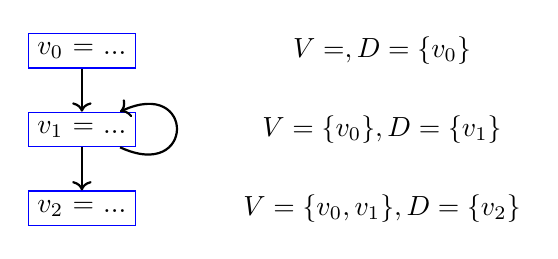
\begin{tikzpicture}
                \node[draw=blue] (head) {$v_0$ = ...};
                \node[draw=blue] (loop) [below of=head] {$v_1$ = ...};
                \node[draw=blue] (tail) [below of=loop] {$v_2$ = ...};
                \draw[->,thick] (head) -- (loop);
                \draw[->,thick] (loop) to [out=-25,in=25,looseness=6] (loop);
                \draw[->,thick] (loop) -- (tail);

                \node<2-> [right of=head, xshift=8em] {$V = \varnothing, D = \{ v_0 \}$};
                \node<3-> [right of=loop, xshift=8em] {$V = \{ v_0 \}, D = \{ v_1 \}$};
                \node<4-> [right of=tail, xshift=8em] {$V = \{ v_0, v_1 \}, D = \{ v_2 \}$};
            \end{tikzpicture}
        \end{block}

    \end{frame}

    \begin{frame}[containsverbatim]{stage 3 --- Building an Analysis}
        \begin{alertblock}{Pass Registration}
        {
        \footnotesize
        \lstinputlisting[breaklines=false,linerange={91-96},language=c++]{../ReachableIntegerValues/ReachableIntegerValues.cpp}
        }
        \end{alertblock}

        \begin{block}{\texttt{CMakeLists.txt}}
        {
        \footnotesize
        \lstinputlisting[breaklines=true,linerange={1-1},language=c++]{../ReachableIntegerValues/CMakeLists.txt}
        }
        \end{block}

    \end{frame}

    \begin{frame}[containsverbatim]{stage 3 --- Analysis}

        \begin{itemize}
            \item Need to export the class declaration in a header
            \item Need to load the analysis in \Command{opt} explicitly
            \item Result of the analysis stored as a member variable
        \end{itemize}

        \structure{API}\\
        {
        \footnotesize
        \lstinputlisting[breaklines=true,linerange={14-16},language=c++]{../include/ReachableIntegerValues.h}
        }
    \end{frame}

    \begin{frame}[containsverbatim]{stage 3 --- Make Result Available}
        \begin{alertblock}{Dependency Processing}
            \begin{enumerate}
                \item PM runs each required analysis (if not cached)
                \item PM runs the Pass entry point
                \item the Pass calls \Code{getAnalysis<\dots>} to access the instance
            \end{enumerate}
        \end{alertblock}
    \end{frame}


    \begin{frame}[containsverbatim]{stage 3 --- Declare Dependencies}

        \begin{alertblock}{Dependency on DominatorTree}
        {
        \footnotesize
        \lstinputlisting[breaklines=true,linerange={80-83},language=c++]{../ReachableIntegerValues/ReachableIntegerValues.cpp}
        }
        \end{alertblock}

    \end{frame}

    \begin{frame}[containsverbatim]{stage 3 --- \texttt{runOnFunction}}
        \begin{alertblock}{Entry Point}
        {
        \footnotesize
        \lstinputlisting[breaklines=true,linerange={21-21,24-24},language=c++]{../ReachableIntegerValues/ReachableIntegerValues.cpp}
        \texttt{~~~//\dots init stuff}
        \lstinputlisting[breaklines=true,linerange={43-44},language=c++]{../ReachableIntegerValues/ReachableIntegerValues.cpp}
        \texttt{~~~//\dots fill the map}
        \lstinputlisting[breaklines=true,linerange={73-74},language=c++]{../ReachableIntegerValues/ReachableIntegerValues.cpp}
        }
        \end{alertblock}
    \end{frame}

    \begin{frame}[containsverbatim]{stage 3 --- Bonus}
        \framesubtitle{LLVM's coding standard}

        \alert{Optional}: You're working out-of tree.\\
        But\dots
        \begin{itemize}
            \item Provides a common reference
            \item Helps for visual consistency
        \end{itemize}
        {
            \footnotesize
\begin{lstlisting}[language=bash]
% find . \( -name '*.cpp' -o -name '*.h' \) \
    -exec clang-format-3.7 -i {} \;
\end{lstlisting}
        }
        \url{http://llvm.org/docs/CodingStandards.html}

    \end{frame}


    %%%%%%%%%%%%%%%%%%%%%%%%%%%%%%%%%%%%%%%
    %%%%%%%%%%%%%%%%%%%%%%%%%%%%%%%%%%%%%%%
    %%%%%%%%%%%%%%%%%%%%%%%%%%%%%%%%%%%%%%%

    \begin{frame}{stage 4}

        \framesubtitle{Write a Complex Pass}

        \begin{block}{Goals}
            \begin{itemize}
                \item Modify the Control Flow Graph (CFG)
                \item Syndicate code in a third-party library
            \end{itemize}

        \end{block}

        \begin{alertblock}{Bonus}
            \begin{itemize}
                \item Declare extra options
                \item Fuzz your passes
                \item Add a support library
            \end{itemize}
        \end{alertblock}

    \end{frame}

    \begin{frame}{stage 4 --- Duplicate basic Blocks}
        \begin{columns}[T]
                \begin{column}{.5\textwidth}
                    \centering
                    \structure{Before}\\\vspace{1em}
                    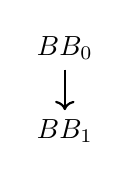
\begin{tikzpicture}[node distance=3em]
                        \node (head) {$BB_0$};
                        \node (cont) [below of=head] {$BB_1$};
                        \draw[->, thick] (head) -- (cont);
                    \end{tikzpicture}
                \end{column}
                \begin{column}{.5\textwidth}
                    \centering
                    \structure{After}\\\vspace{1em}
                    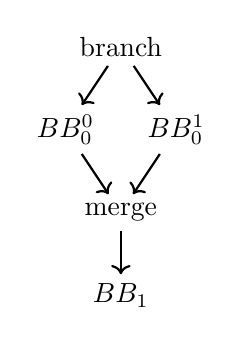
\begin{tikzpicture}[node distance=3em]
                        \node (cond) {branch};
                        \node (clone0) [below of=cond, xshift=-2em] {$BB_0^0$};
                        \node (clone1) [below of=cond, xshift=+2em] {$BB_0^1$};
                        \node (merge) [below of=clone1, xshift=-2em] {merge};
                        \node (cont) [below of=merge] {$BB_1$};
                        \draw[->, thick] (cond) -- (clone0);
                        \draw[->, thick] (cond) -- (clone1);
                        \draw[->, thick] (clone0) -- (merge);
                        \draw[->, thick] (clone1) -- (merge);
                        \draw[->, thick] (merge) -- (cont);
                    \end{tikzpicture}
                \end{column}
        \end{columns}

    \end{frame}

    \begin{frame}{stage 4 --- Problems}
        \begin{itemize}
            \item Cloning \Code{BasicBlock}s and iterating over a function loops
            \item Cloning an instruction creates a new \Code{Value}
            \item Cloning several instructions requires a remapping
        \end{itemize}
    \end{frame}

    \begin{frame}{stage 4 --- Messing with $\varphi$s}
        \begin{enumerate}
            \item Forge a random condition using result of \Code{ReachableIntegerValues}
            \item Clone a \Code{BasicBlock}
            \item Merge \Code{Value}s from the clones using $\varphi$ nodes
        \end{enumerate}
        $\Rightarrow$ Using a \Code{FunctionPass}
    \end{frame}

    \begin{frame}[containsverbatim]{stage 4 --- Forge a Random Branch}

        \structure{Get analysis result}\\
        \begin{minipage}{\textwidth}
        \scriptsize
        \lstinputlisting[breaklines=false,linerange={73-74},language=c++]{../DuplicateBB/DuplicateBB.cpp}
        \end{minipage}

        \structure{Pick a random reachable value}\\
        \hspace{-2em}%
        \begin{minipage}{\textwidth}
        \scriptsize
        \lstinputlisting[breaklines=false,linerange={87-89},language=c++]{../DuplicateBB/DuplicateBB.cpp}
        \end{minipage}

        \structure{Random condition}\\
        \begin{minipage}{\textwidth}
        \scriptsize
        \lstinputlisting[breaklines=false,linerange={125-128},language=c++]{../DuplicateBB/DuplicateBB.cpp}
        \end{minipage}
    \end{frame}

    \begin{frame}[containsverbatim]{stage 4 --- Messing with Clones}
        \structure{Cloning an instruction}\\
        \hspace{-2em}%
        \begin{minipage}{\textwidth}
        \scriptsize
        \lstinputlisting[breaklines=false,linerange={169-170},language=c++]{../DuplicateBB/DuplicateBB.cpp}
        \end{minipage}

        \structure{Remap operands}\\
        \hspace{-2em}%
        \begin{minipage}{\textwidth}
        \scriptsize
        \lstinputlisting[breaklines=false,linerange={172-172},language=c++]{../DuplicateBB/DuplicateBB.cpp}
        \end{minipage}

        \structure{Manual $\varphi$ creation}\\
        \hspace{-2em}%
        \begin{minipage}{\textwidth}
        \scriptsize
        \lstinputlisting[breaklines=false,linerange={183-185},language=c++]{../DuplicateBB/DuplicateBB.cpp}
        \end{minipage}

    \end{frame}

    \begin{frame}[containsverbatim]{stage 4 --- Bonus}
        \framesubtitle{Fuzz your creation}
        \begin{alertblock}{Using \Command{csmith}}
            \begin{enumerate}
                \item Pick \url{http://embed.cs.utah.edu/csmith/}
                \item Write configuration file, e.g. \Command{fuzz.cfg}:
                    {
                        \scriptsize
\begin{lstlisting}[language=bash]
clang -O2
clang -O2 -Xclang -load -Xclang LLVMDuplicateBB.so
\end{lstlisting}
                    }
                \item Run generation!
                    {
                        \scriptsize
\begin{lstlisting}[language=bash]
% CSMITH_HOME=$PWD ./scripts/compiler_test.pl 1000 fuzz.cfg
\end{lstlisting}
                    }
            \end{enumerate}
        \end{alertblock}
    \end{frame}

    \begin{frame}[containsverbatim]{stage 4 --- Bonus}
        \framesubtitle{Add extra options}
        \begin{alertblock}{Control the obfuscation ratio}
        {
        \scriptsize
        \lstinputlisting[breaklines=false,linerange={32-39},language=c++]{../DuplicateBB/DuplicateBB.cpp}
        }
        \end{alertblock}
        \vspace{.1em}
        \structure{$\Rightarrow$} Need to specialize \Code{llvm:cl} for the \Code{Ratio} class.
    \end{frame}


    \begin{frame}{stage 4 --- Bonus}
        \framesubtitle{Add a support library}
        \begin{alertblock}{\Code{CMakeLists.txt}}
            \begin{minipage}{\textwidth}
            \scriptsize
            \lstinputlisting[breaklines=false,linerange={3-3},language=bash]{../DuplicateBB/CMakeLists.txt}
            \end{minipage}
        \end{alertblock}

        \begin{alertblock}{Specialize \Code{llvm::cl::parser}}
            \begin{minipage}{\textwidth}
            \scriptsize
            \lstinputlisting[breaklines=false,linerange={22-25},language=c++]{../include/Utils.h}
            \end{minipage}
        \end{alertblock}
    \end{frame}
    %%%%%%%%%%%%%%%%%%%%%%%%%%%%%%%%%%%%%%%
    %%%%%%%%%%%%%%%%%%%%%%%%%%%%%%%%%%%%%%%
    %%%%%%%%%%%%%%%%%%%%%%%%%%%%%%%%%%%%%%%

    \begin{frame}{Final Boss}
        \only<1>{
        \begin{center}
            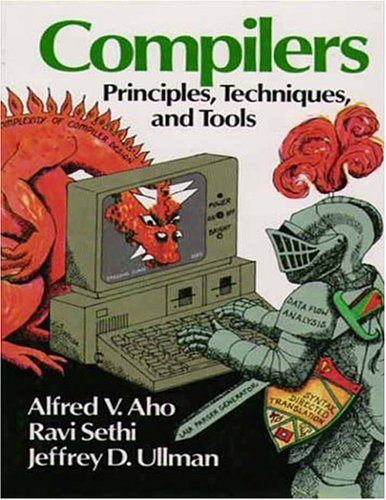
\includegraphics[width=.4\textwidth]{dragon_book.jpg}
        \end{center}
        }
        \only<2>{
        \begin{tikzpicture}
            \node[rotate=-45] at (3,2) {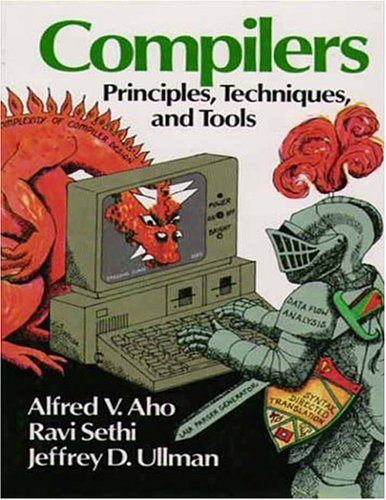
\includegraphics[width=.2\textwidth]{dragon_book.jpg}};
            \node[rotate=-80] at (5,3.5) {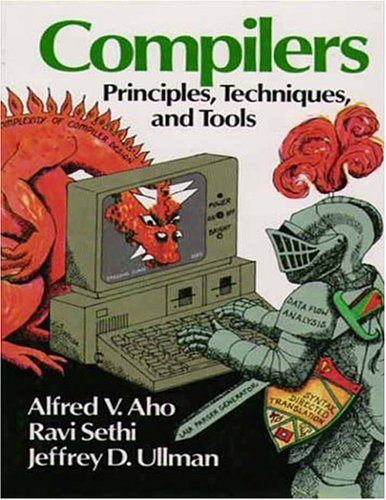
\includegraphics[width=.1\textwidth]{dragon_book.jpg}};
            \node[rotate=-105] at (6,4.4) {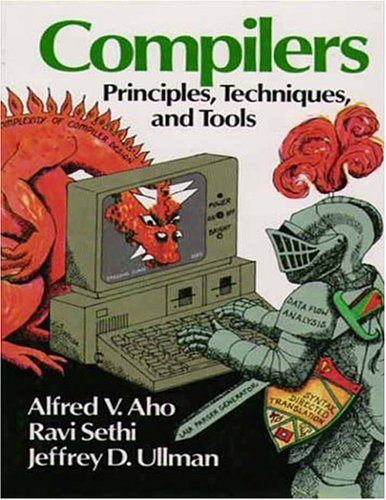
\includegraphics[width=.05\textwidth]{dragon_book.jpg}};
            \node[rotate=-125] at (7,5.2) {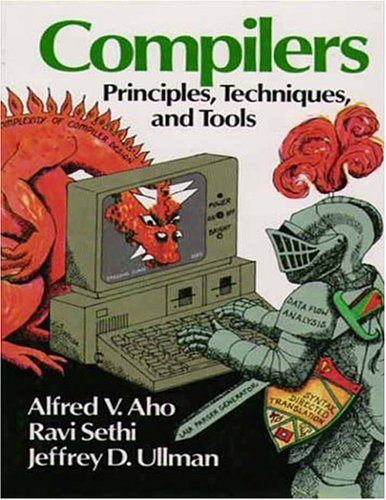
\includegraphics[width=.025\textwidth]{dragon_book.jpg}};
            \node[rotate=-45] at (3,2) {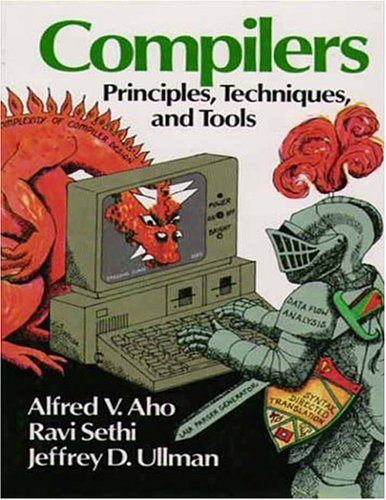
\includegraphics[width=.2\textwidth]{dragon_book.jpg}};
            \node at (0,0) {
\includegraphics[width=.5\textwidth]{dragon_punch.png}};
        \end{tikzpicture}
        }

    \end{frame}


    %%%%%%%%%%%%%%%%%%%%%%%%%%%%%%%%%%%%%%%
    %%%%%%%%%%%%%%%%%%%%%%%%%%%%%%%%%%%%%%%
    %%%%%%%%%%%%%%%%%%%%%%%%%%%%%%%%%%%%%%%

    \begin{frame}{GAME OVER}

        \begin{itemize}
            \centering
            \item[]
\includegraphics[height=2em]{logo.png}
            \item[]\alert{\bf Creditz}\vspace{-1em}
            \item[]\texttt{Serge~Guelton~<sguelton@quarkslab.com>}
            \item[]\texttt{Adrien Guinet <aguinet@quarkslab.com>}
        \end{itemize}
        %
        \begin{itemize}
            \centering
            \item[]\alert{\bf Insert Coins}\vspace{.1em}
            \item[]\texttt{Exit}
            \item[]\texttt{\hyperlink{page.1}{> Play Again <}}
        \end{itemize}

    \end{frame}

\end{document}
